
\section{Community Support Study (RQ2)}
\label{sec:rq2}
The goal of this evaluation is to understand how frequently each of the regex representations appears in the source code, as a way to identify community standards code smells~\cite{stoleeicse, stoleeTSE}. %. Based on the results, we identify preferred representations using popularity in the source code.



\subsection{Artifacts}
We analyzed an existing
corpus of regexes collected from Python code in GitHub projects~\cite{chapman2016}.
This dataset has 13,597 distinct (non-duplicate) regex patterns from 1,544 projects.

%We targeted Python as it is a popular programming language with a strong presence on GitHub, being the fourth most common language after Java, Javascript, and Ruby. Further, Python's regex pattern language is close enough to other regex libraries that our conclusions are likely to generalize.
This corpus was created by analyzed static invocations to the Python {\tt re} library.
Consider the Python snippet:
\begin{lstlisting}[language=Python,firstnumber=1, basicstyle=\footnotesize]
r1 = re.compile('(0|-?[1-9][0-9]*)$', re.MULTILINE)
\end{lstlisting}
The \emph{function} {\tt re.compile} returns a regex object {\tt r1}.
The \emph{pattern}, \verb!(0|-?[1-9][0-9]*)$, !defines what strings will be matched and the \emph{flag} {\tt re.MULTILINE} modifies the matching behavior.
%The regex pattern is an ordered series of regular expression language feature tokens.
This particular regex will match strings with a zero at the end of a line, or an integer at the end of a line (i.e., the {\tt -?} sequence indicates the integer may be negative).


%Our goal was to collect regex patterns from a variety of projects to represent the breadth of how developers use regexes.
%We scraped 3,898 projects containing Python code using the GitHub API. This was done by systematically selecting repository IDs, checking the repository for Python files, and retaining the project if Python was found. After dividing eight million repository IDs into 32 groups, we scanned from the beginning until we had collected approximately four thousand Python projects.
%%We did so by dividing a range of about 8 million repo IDs
%%into 32 sections of equal size and scanning for Python projects from the beginning of those
%%segments until we ran out of memory.
%At that point, we felt we had enough data
%to do an analysis without further perfecting our mining techniques.
%
%To identify invocations of the {\tt re} module, we built
%the AST of each Python file in each project. In most projects, almost all {\tt re} invocations are present in the
%most recent version of a project, but to be more thorough, we also scanned up
%to 19 earlier versions.
%%The number 20 was chosen to try and maximize returns on
%%computing resources invested after observing the scanning process in many hours
%%of trial scans.
%% If the project had fewer than 20 commits, then all commits were scanned.
%% The most recent commit was always included, and the spacing between all other chosen commits was determined by dividing the remaining number of commits by 19 (rounding as needed).
%All regex patterns were retained, sans duplicates.
%%Within a project, a duplicate utilization was marked when two versions of the same file have the same function, pattern, and flags.
%In the end, we observed and recorded 16,088 non-duplicate patterns in 1,645 projects.
%%\todoLast{1544 may be a white lie...the 13K+ patterns come from 1544 projects, but the 54k utilizations (before pruning) probably come from something like 1900 projects, and that number is somewhere in the git history of tour de source}
%
%In collecting the set of distinct patterns for analysis, we ignore the 12.7\% of {\tt re} invocations using flags, which can alter regex behavior. An additional 6.5\% of {\tt re} invocations contained patterns that could not be compiled because the pattern was non-static (e.g., used some runtime variable).
%%The remaining 80.8\% (43,525) of the utilizations were collapsed into 13,711 distinct pattern strings.
%This parser was unable to support 0.8\% (114) due to error.
%% of the patterns due to unsupported Unicode characters. Another 0.2\% (25) of the patterns used regex features that we chose to exclude because they appeared very rarely (e.g., reference conditions). An additional 0.1\% (16) of the patterns were excluded because they were empty or otherwise malformed so as to cause a parsing error.




\subsection{Metrics}
\label{sec:communitymetric}
We measure community support by matching regexes in the corpus to representations in Figure~\ref{fig:refactoringTree} and counting the \emph{patterns} and \emph{projects}. These are referred to as the \emph{community standards metrics}.
%A \emph{pattern} is extracted from a utilization, as shown in Figure~\ref{fig:exampleUsage}.
A regex can belong to multiple representations and to multiple projects since the corpus tracked duplicates.
% and only analyze the distinct regex patterns.

% that represent 43,525 regex utilizations across the projects.\todoMid{feels weird to hear this again right away, maybe simplify the metrics paragraph}
%For this frequency analysis, we focus on patterns and the number of projects the patterns appear in.
%To determine how often each representation appears in the wild, we extract regex patterns from source code and measure if a representation matches (part of) the pattern.
%
%
%\paragraph{Patterns}



%\paragraph{Projects}

%The process for deciding if a particular pattern belongs to a particular node is described in detail in Section~\ref{communityanalysis}.


\subsection{Analysis}
\label{communityanalysis}
To match patterns to representations, we used the PCRE parser or treated the regexes as token streams, depending on the characteristics of the representation. Our analysis code is available on GitHub\footnote{\url{https://github.com/wangpeipei90/RegexSmells}}.
%To match patterns to representations, we used the PCRE parser or treated the regexes as token streams, depending on the characteristics of the representation. Our analysis code is available on GitHub\footnote{blinded for review}. %\url{http://tinyurl.com/jmeeytk} (this is a git repo - not anonymized)}.
Next, we describe the process in detail:

\subsubsection{Presence of a Feature}
For representations that require a particular feature, we used the PCRE parser to decide membership. This applies to D1 (double-bounded repetition with different bounds), D2 (question-mark), S1 (single-bounded repetition), S3 (double-bounded repetition with the same bounds), L1 (lower-bound repetition), L2 (Kleene star), L3 (add repetition), and C3 (negated custom character class).

%
%\begin{figure}[tb]
%\centering
%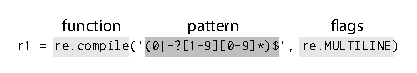
\includegraphics[width=\columnwidth]{illustrations/exampleUsage.eps}
%\vspace{-12pt}
%\caption{Example Python regex library invocation (credit: Chapman and Stolee~\cite{chapman2016})}
%\vspace{-6pt}
%\label{fig:exampleUsage}
%\end{figure}


\begin{table*}[ht]
\begin{small}\begin{center}
\caption{How frequently is each alternative expression style used?}
\label{table:nodeCount}
\begin{tabular}
{lll@{}rrrr}
name & description & example & nPatterns & \% patterns & nProjects & \% projects \\
\toprule[0.16em]
C1 & char class using ranges & \begin{minipage}{1.5in}\begin{verbatim}
'^[1-9][0-9]*$'\end{verbatim}\end{minipage}
 & 2,479 & 18.2\% & 810 & 52.5\%\\
C2 & char class explicitly listing all chars & \begin{minipage}{1.5in}\begin{verbatim}
'[aeiouy]'\end{verbatim}\end{minipage}
 & 1,283 & 9.4\% & 551 & 35.7\%\\
C3 & any negated char class & \begin{minipage}{1.5in}\begin{verbatim}
'[^A-Za-z0-9.]+'\end{verbatim}\end{minipage}
 & 1,935 & 14.2\% & 776 & 50.3\%\\
C4 & char class using defaults & \begin{minipage}{1.5in}\begin{verbatim}
'[-+\d.]'\end{verbatim}\end{minipage}
 & 840 & 6.2\% & 414 & 26.8\%\\
C5 & an OR of length-one sub-patterns & \begin{minipage}{1.5in}\begin{verbatim}
'(@|<|>|-|!)'\end{verbatim}\end{minipage}
 & 245 & 1.8\% & 239 & 15.5\%\\
\midrule
D1 & curly brace repetition like \{M,N\} with M<N & \begin{minipage}{1.5in}\begin{verbatim}
'^x{1,4}$'\end{verbatim}\end{minipage}
 & 367 & 2.7\% & 242 & 15.7\%\\
D2 & zero-or-one repetition using question mark & \begin{minipage}{1.5in}\begin{verbatim}
'^http(s)?://'\end{verbatim}\end{minipage}
 & 1,871 & 13.8\% & 646 & 41.8\%\\
D3 & repetition expressed using an OR & \begin{minipage}{1.5in}\begin{verbatim}
'^(Q|QQ)\<(.+)\>$'\end{verbatim}\end{minipage}
 & 10 & .1\% & 27 & 1.7\%\\
\midrule
T1 & no HEX, OCT or char-class-wrapped literals & \begin{minipage}{1.5in}\begin{verbatim}
'get_tag'\end{verbatim}\end{minipage}
 & 12,482 & 91.8\% & 1,485 & 96.2\%\\
T2 & has HEX literal like \verb!\xF5! & \begin{minipage}{1.5in}\begin{verbatim}
'[\x80-\xff]'\end{verbatim}\end{minipage}
 & 479 & 3.5\% & 243 & 15.7\%\\
T3 & has char-class-wrapped literals like [\$] & \begin{minipage}{1.5in}\begin{verbatim}
'[$][{]\d+:([^}]+)[}]'\end{verbatim}\end{minipage}
 & 307 & 2.3\% & 268 & 17.4\%\\
T4 & has OCT literal like \verb!\0177! & \begin{minipage}{1.5in}\begin{verbatim}
'[\041-\176]+:$'\end{verbatim}\end{minipage}
 & 14 & .1\% & 37 & 2.4\%\\
\midrule
L1 & curly brace repetition like \{M,\} & \begin{minipage}{1.5in}\begin{verbatim}
'(DN)[0-9]{4,}'\end{verbatim}\end{minipage}
 & 91 & .7\% & 166 & 10.8\%\\
L2 & zero-or-more repetition using kleene star & \begin{minipage}{1.5in}\begin{verbatim}
'\s*(#.*)?$'\end{verbatim}\end{minipage}
 & 6,017 & 44.3\% & 1,097 & 71.0\%\\
L3 & one-or-more repetition using plus & \begin{minipage}{1.5in}\begin{verbatim}
'[A-Z][a-z]+'\end{verbatim}\end{minipage}
 & 6,003 & 44.1\% & 1,207 & 78.2\%\\
\midrule
S1 & curly brace repetition like \{M\} & \begin{minipage}{1.5in}\begin{verbatim}
'^[a-f0-9]{40}$'\end{verbatim}\end{minipage}
 & 581 & 4.3\% & 340 & 22.0\%\\
S2 & explicit sequential repetition & \begin{minipage}{1.5in}\begin{verbatim}
'ff:ff:ff:ff:ff:ff'\end{verbatim}\end{minipage}
 & 3,378 & 24.8\% & 861 & 55.8\%\\
S3 & curly brace repetition like \{M,M\} & \begin{minipage}{1.5in}\begin{verbatim}
'U[\dA-F]{5,5}'\end{verbatim}\end{minipage}
 & 27 & .2\% & 32 & 2.1\%
 \\
\bottomrule[0.13em]
\end{tabular}
\end{center}\end{small}\end{table*}



\subsubsection{Features and Pattern}
%The presence of a feature is not always enough to determine membership.
%However, the presence of a feature and properties of the pattern can determine membership.
Identifying D3 requires an OR containing at least two entries with a sequence present in one entry repeated N times and the same sequence present in another entry repeated N+1 times. We first looked for a sequence of N repeating groups with an OR-bar (i.e., \verb!|!) next to them on a side. This produced a list of 113 candidates which we narrowed down manually to 10 actual members.


T2 requires a literal with a hex structure. %that matches the regex \verb!(\\x[a-f0-9A-F]{2})! which reliably identifies hex codes within a pattern.
T4 requires a literal with a %and must match the regex \verb!((\\0\d*)|(\\\d{3}))! which is specific to
Python-style octal structure. %, requiring either exactly three digits after a slash, or a zero and some other digits after a slash. One false positive was identified, which was actually the lower end of a hex range using the literal \verb!\0!.
T3 requires that a single literal character is wrapped in a custom character class (a member of T3 is always a member of C2).
T1 requires that no characters are wrapped in brackets or are hex or octal characters, which matches over 91\% of the patterns analyzed.

\subsubsection{Token Stream }
%The rest of the representations were identified by representing the regex patterns as a sequence of tokens.
S2 requires a repeated element. This element could be a character class, a literal, or a collection of things encapsulated in parentheses; rather than a parser, we used a token stream to identify it.
C1 requires that a non-negative character class contains a range.
C2 requires that there exists a custom character class that does not use ranges or defaults.
C4 requires the presence of a default character class within a custom character class.
%, specifically, \verb!\d!, \verb!\D!, \verb!\w!, \verb!\W!, \verb!\s!, \verb!\S! and \verb!.!.
C5 requires an OR of length-one sequences (literal characters or any character class).


\subsection{Results}
Table~\ref{table:nodeCount} presents the results.
% frequencies with which each representation appears in a regex pattern and in a project scraped from GitHub.
 \emph{Node} references Figure~\ref{fig:refactoringTree}, \emph{description} briefly describes the representation, \emph{example} provides a regex from the corpus. \emph{nPatterns} counts the patterns that belong to the representation, followed by the percent of patterns out of 13,597.
 \emph{nProjects} counts the projects that contain a regex belonging to the representation,
followed by the percentage of projects out of 1,544.
%The project support is used to show pervasiveness across the whole corpus.
For example, D1 appears in 346 (2.5\%) of the patterns but only 234 (15.2\%) of the projects.
 In contrast, T3 appears in 39 \emph{fewer} patterns but 34 \emph{more} projects, indicating that D1 is more concentrated in a few projects and T3 is more widespread across projects.

The pattern frequency is our guide for setting the community standards.
For example, since C1 is more prevalent than C2 in both patterns and projects, we could say that C2 is smelly since it could better conform to community standards if expressed as C1.
%Based on patterns alone, the winning representations per equivalence class are C1, D2, T1, L2, and S2. With one exception, these are the same for recommendations based on projects; L3 appears in more projects than L2, so it is unclear which is smelly.

%Our analysis simply suggests smells. %a direction for a refactoring (in this case, from C4 to C1).
%Section~\ref{sec:rq3} explores these results more deeply.

%Table~\ref{summaryResults} presents these recommendations for each pair of representations within each equivalence class. The \emph{Comm} column is populated based on the findings of \emph{RQ1}. The findings for \emph{RQ2} and \emph{RQ3} are in the \emph{Match} and \emph{Compose} columns, respectively.

\subsection{Summary}
Based on patterns, the winning representations per equivalence class are C1, D2, T1, L2, and S2. With one exception, these are the same project-based recommendations; L3 appears in more projects than L2, so it is unclear which is smelly.
